\chapter{Web App}\label{ch:web-app}

This chapter of the report will detail the local design and development of the \textit{Digital Ink} web application.
We will first discuss the software stack used to develop the app, then the design of the database used, and, lastly, the design of the user interface.

\section{Software Stack}\label{sec:stack}

\textit{Digital Ink} was first developed locally using a LAMP stack.
LAMP refers to a generic software stack, where each letter in the acronym stands for one the following open source building blocks: Linux, Apache HTTP Server, MySQL, and PHP \parencite{lee2003open}.
The web app is hosted within a Docker container~\parencite{anderson2015docker} which runs a minified version of the Linux operating system.
Apache is an open-source web server software which is used to host the app on the web~\parencite{fielding1997apache}.
MySQL is an open-source relational database management system~\parencite{widenius2002mysql} which is used to store all the data used within the app, including user details and story details.
PHP is a programming language aimed towards web development, chosen due to its stability and reliability~\parencite{lerdorf2002programming}.
Additionally, all developers involved have prior experience with PHP\@.

\section{Database Design}\label{sec:database}

As mentioned before, the web app uses the MySQL relational database management system to store its data.
MySQL is a relational database management system (RDBMS) which stores data in the form of tables, where Structures Query Language (SQL) is used to access the database.
As shown in Figure~\ref{fig:tables-overview}, the database which this web app uses consists of three tables: \mintinline{sql}|users|, \mintinline{sql}|stories|, and \mintinline{sql}|migrations|.

\begin{figure}[!htbp]
    \centering
    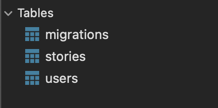
\includegraphics[scale=0.8]{resources/database/tables-overview}
    \caption{Database tables overview.}
    \label{fig:tables-overview}
\end{figure}

The \mintinline{sql}|migrations| table (see Figure~\ref{fig:migrations-records}) contains records which correspond to the migrations within the Laravel web app.
These migrations contain the scripts required to automatically generate the \mintinline{sql}|users| and \mintinline{sql}|stories| tables in SQL\@.
It contains the following three columns:

\begin{itemize}
    \item \mintinline{sql}|id|: the unique ID for each migration.
    \item \mintinline{sql}|migration|: points to the scripts used to create tables.
    \item \mintinline{sql}|batch|: how many times the script has been ran.
\end{itemize}

\begin{figure}[!htbp]
    \centering
    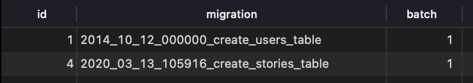
\includegraphics[width=\textwidth]{resources/database/migrations-records}
    \caption{\mintinline{sql}|migrations| table.}
    \label{fig:migrations-records}
\end{figure}

The \mintinline{sql}|users| table (see Figure~\ref{fig:users-records}) contains all the information about user accounts, and it contains the following seven columns:

\begin{itemize}
    \item \mintinline{sql}|id|: the unique ID for each user account.
    \item \mintinline{sql}|name|: the name associated with user account.
    \item \mintinline{sql}|email|: the unique email used to log in.
    \item \mintinline{sql}|password|: the password used to log in, encrypted with 184 bit hashing by Bcrypt~\parencite{laravel2022hashing}.
    \item \mintinline{sql}|remember_token|: keeps the user logged in if they select "Remember me".
    \item \mintinline{sql}|created_at|: records what date and time the user account was first created at.
    \item \mintinline{sql}|updated_at|: records what date and time the user account was last updated at.
\end{itemize}

\begin{figure}[!htbp]
    \centering
    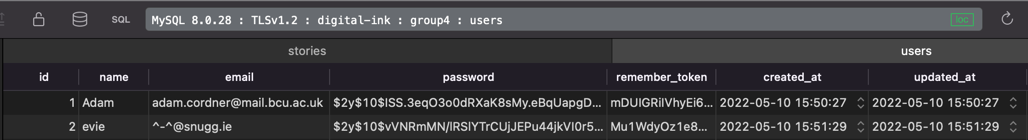
\includegraphics[width=\textwidth]{resources/database/users-records}
    \caption{\mintinline{sql}|users| table.}
    \label{fig:users-records}
\end{figure}

\clearpage
The \mintinline{sql}|stories| table (see Figure~\ref{fig:stories-records}) contains all the information about user-created stories, and it contains the following 11 columns:

\begin{itemize}
    \item \mintinline{sql}|id|: the unique ID for each story.
    \item \mintinline{sql}|author_id|: the unique ID associated with the user who created the story.
    \item \mintinline{sql}|title|: the title associated with the story.
    \item \mintinline{sql}|genre|: the genre associated with the story, which can be one of eight different genres.
    \item \mintinline{sql}|blurb|: a brief description of the story.
    \item \mintinline{sql}|content|: the full content of the story.
    \item \mintinline{sql}|cover_image|: a thumbnail image for the story.
    \item \mintinline{sql}|file_upload|: an optional PDF upload of the story.
    \item \mintinline{sql}|published|: 1 if the story has been made public, or 0 if it is a draft.
    \item \mintinline{sql}|created_at|: records what date and time the story was first created at.
    \item \mintinline{sql}|updated_at|: records what date and time the story was last updated at.
\end{itemize}

\begin{figure}[!htbp]
    \centering
    \begin{subfigure}
        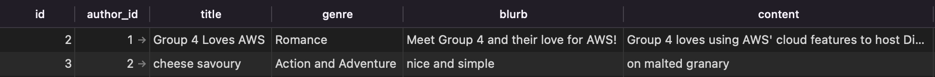
\includegraphics[width=\textwidth]{resources/database/stories-records-1}
    \end{subfigure}
    \begin{subfigure}
        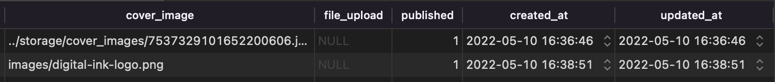
\includegraphics[width=\textwidth]{resources/database/stories-records-2}
    \end{subfigure}
    \caption{\mintinline{sql}|stories| table.}
    \label{fig:stories-records}
\end{figure}

\clearpage
\section{Interface Design}\label{sec:interface}

The design of the web app was created using Blade, a powerful templating engine~\parencite{laravel2022blade}.
When the user initially accesses the web app, they are able to log in or sign up.
This can be seen in Figure~\ref{fig:digital-ink-home-and-sign-up}.
When a user has created an account, a record is written to the \mintinline{sql}|users| table in the database.

\begin{figure}[!htbp]
    \centering
    \begin{minipage}{.5\textwidth}
        \centering
        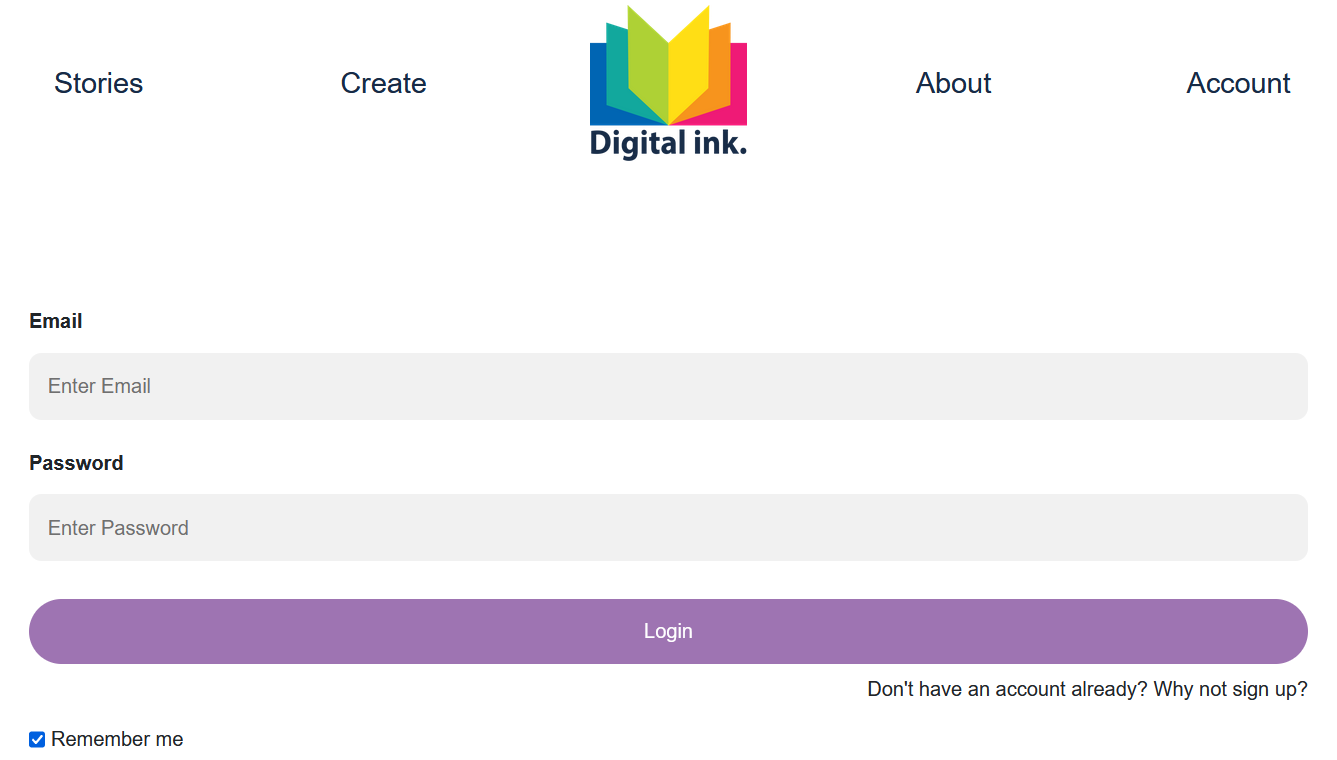
\includegraphics[width=1\linewidth]{resources/webapp/digital-ink-home}
        \label{fig:digital-ink-home}
    \end{minipage}%
    \begin{minipage}{.5\textwidth}
        \centering
        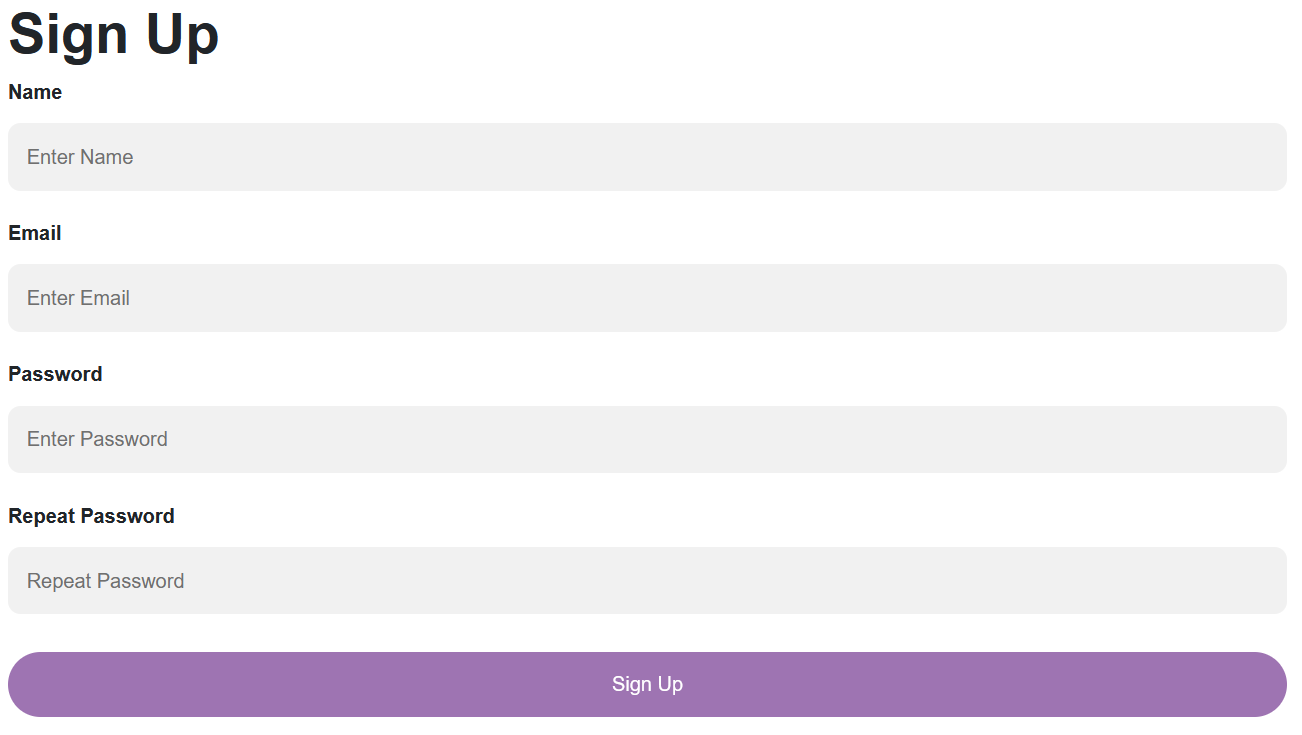
\includegraphics[width=1\linewidth]{resources/webapp/digital-ink-sign-up}
        \label{fig:digital-ink-sign-up}
    \end{minipage}
    \caption{\textit{Digital-Ink} home page log in and sign up forms.}
    \label{fig:digital-ink-home-and-sign-up}
\end{figure}

\clearpage
Once a user is signed in, they can create a story.
Creating a story requires the user to entire a title, a genre, the story itself, a blurb, and, optionally, a thumbnail image.
This can be seen in Figure~\ref{fig:digital-ink-create-story}.
Once a story has been created, it is written to the \mintinline{sql}|stories| table.

\begin{figure}[!htbp]
    \centering
        \begin{subfigure}
            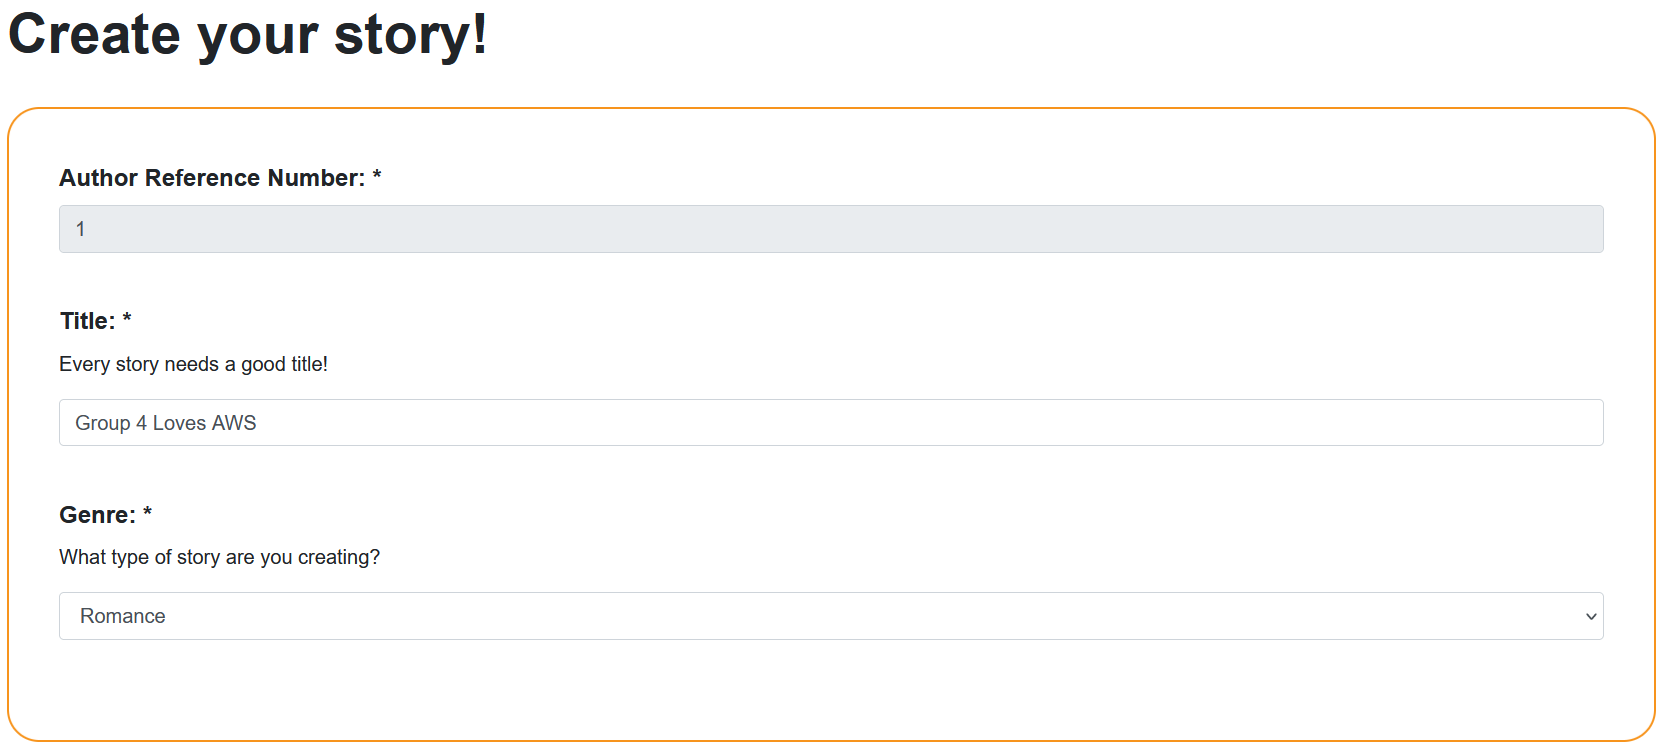
\includegraphics[width=\textwidth]{resources/webapp/digital-ink-create-story-1}
        \end{subfigure}
        \begin{subfigure}
            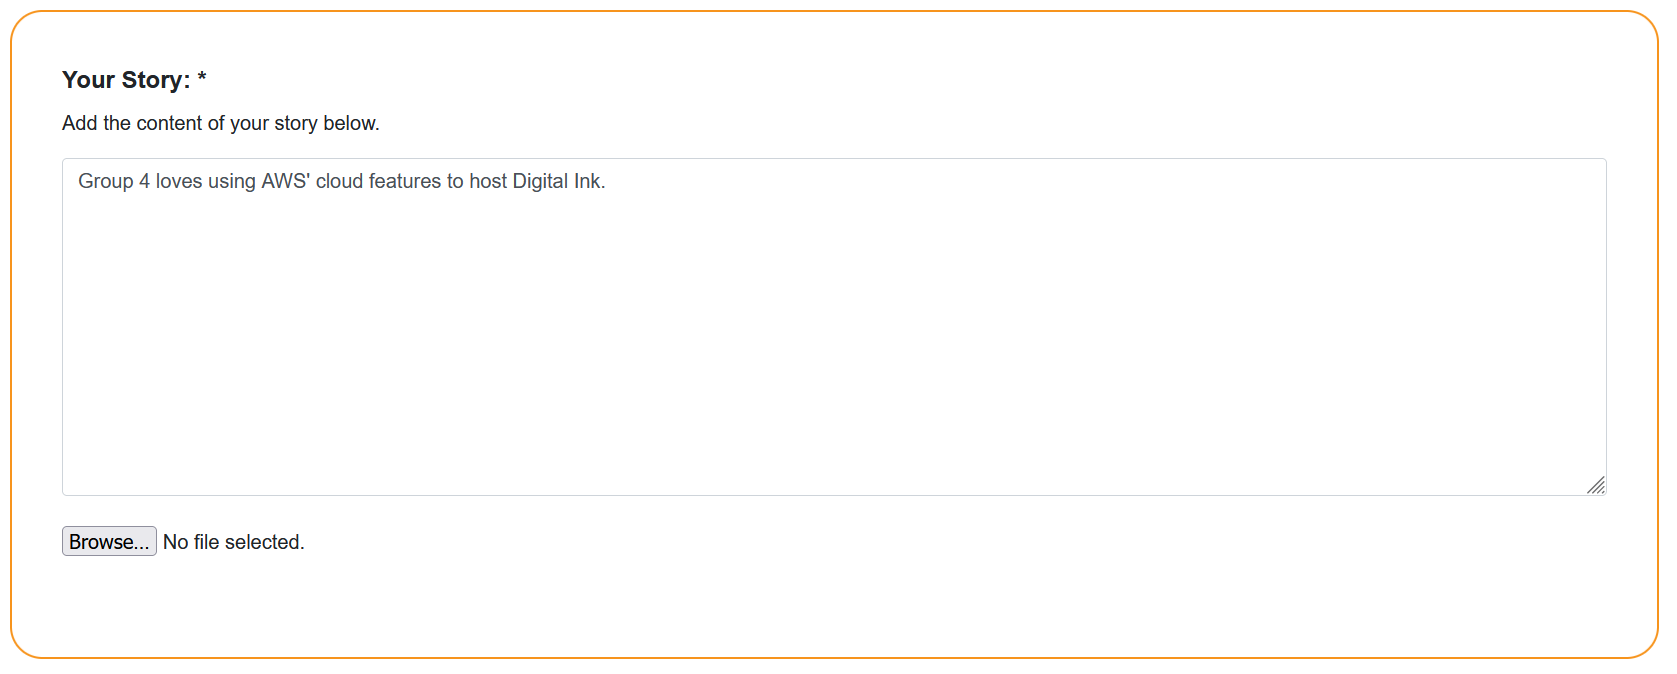
\includegraphics[width=\textwidth]{resources/webapp/digital-ink-create-story-2}
        \end{subfigure}
        \begin{subfigure}
            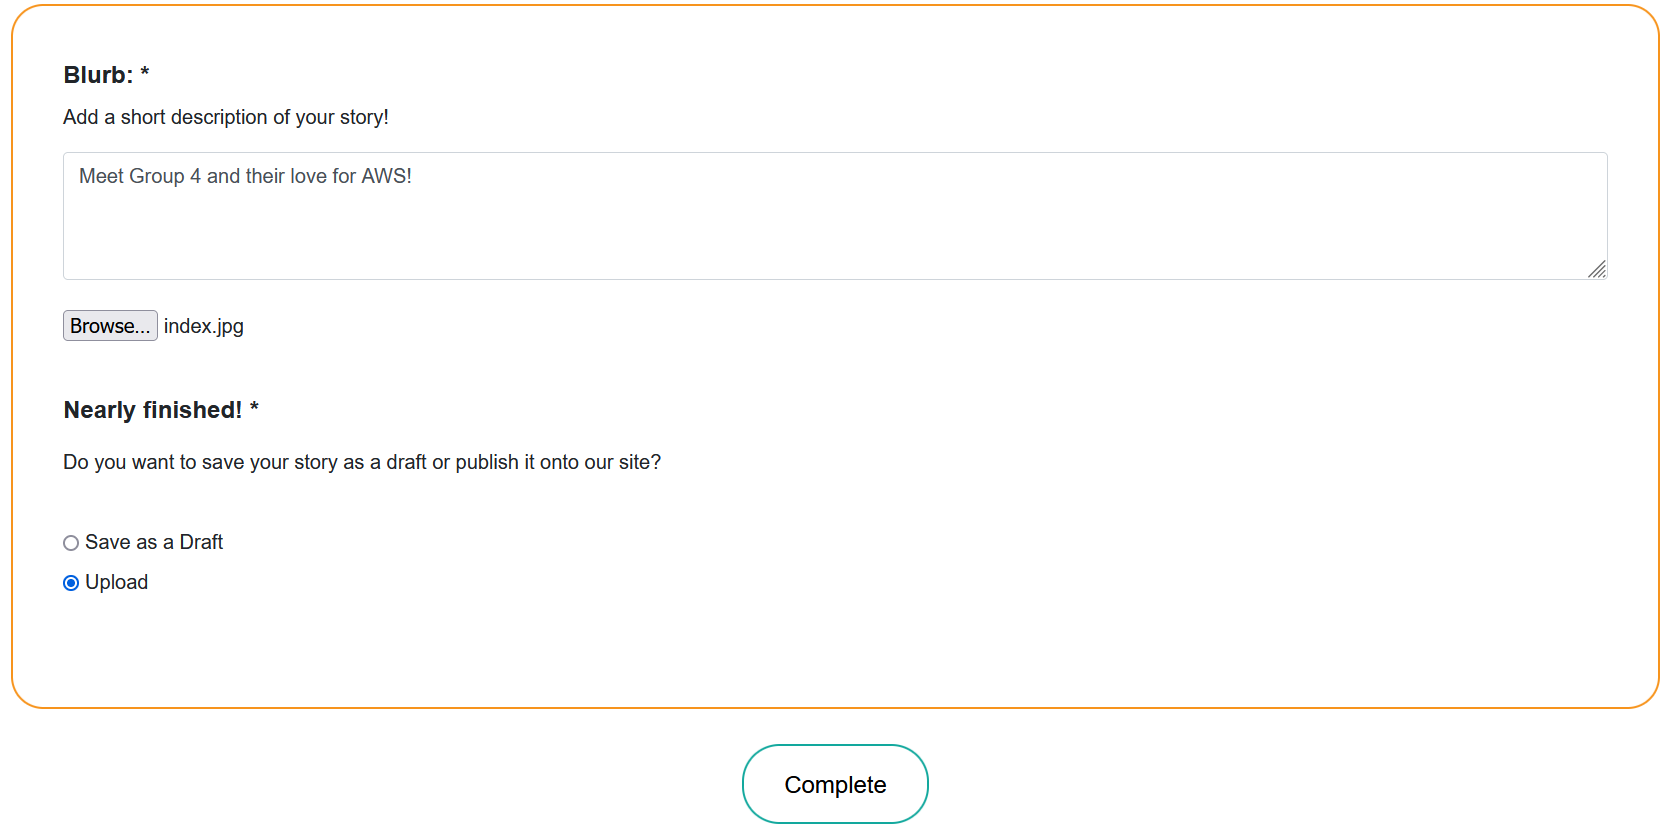
\includegraphics[width=\textwidth]{resources/webapp/digital-ink-create-story-3}
        \end{subfigure}
        \caption{\textit{Digital-Ink} story creation form.}
        \label{fig:digital-ink-create-story}
\end{figure}

\clearpage
After this, the user can see all of their uploaded stories on their account page.
This can be seen in Figure~\ref{fig:digital-ink-account}.
From here, a story can be edited or deleted, which either updates a record in the \mintinline{sql}|stories|table or removes a record from it.

\begin{figure}[!htbp]
    \centering
        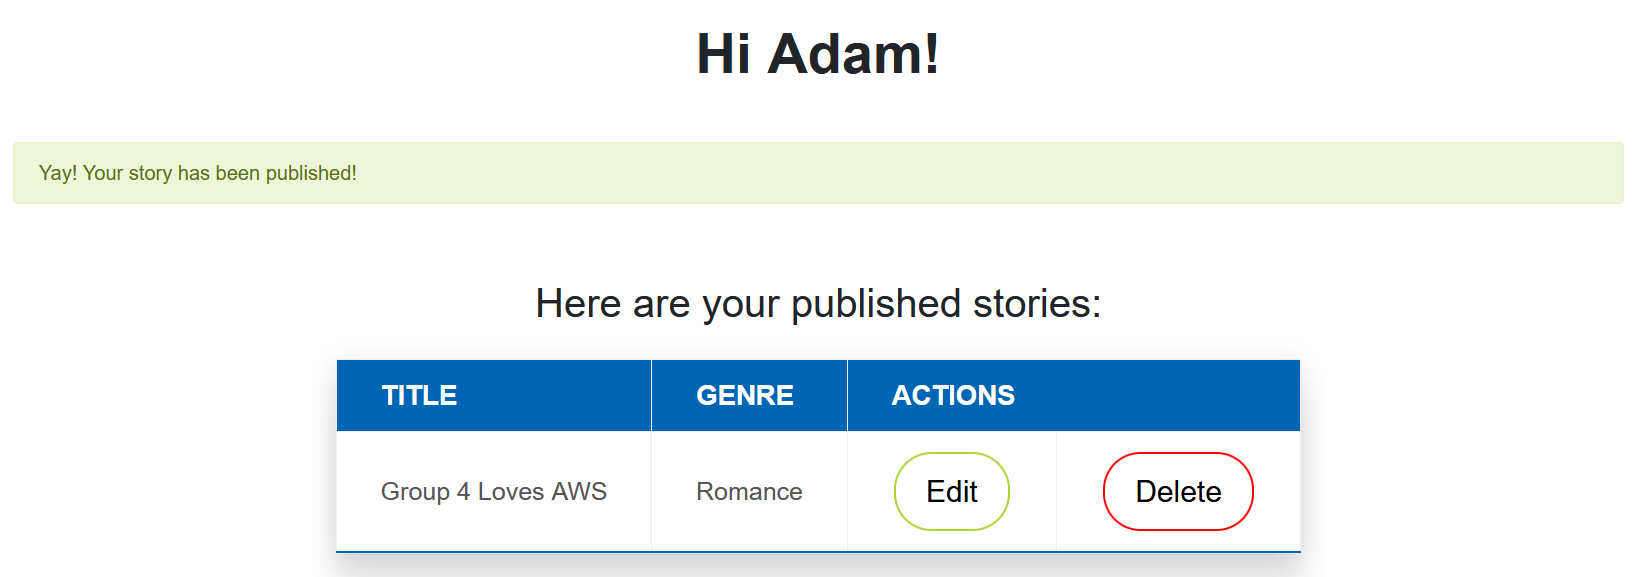
\includegraphics[width=\textwidth]{resources/webapp/digital-ink-account}
        \caption{\textit{Digital-Ink} account page.}
        \label{fig:digital-ink-account}
\end{figure}

Lastly, on the Stories page, a user can view and search through all uploaded stories across all users.
Each story's title, genre, and blurb is shown in a list view.
A user can click into one of these stories to see the thumbnail image and read the full story.
These pages can be seen in Figure~\ref{fig:digital-ink-stories-and-story}.

\begin{figure}[!htbp]
    \centering
    \begin{subfigure}
        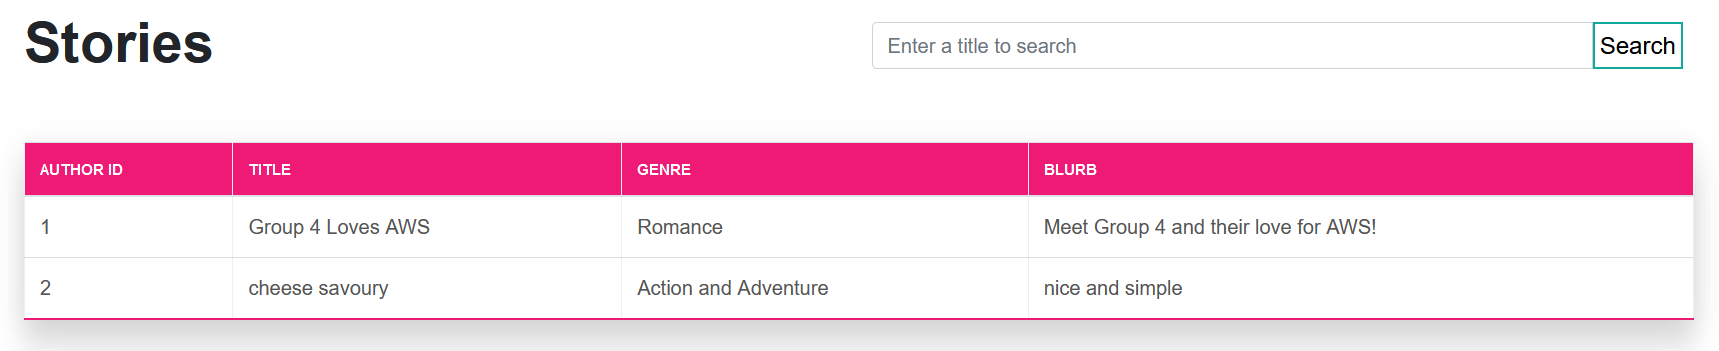
\includegraphics[width=\textwidth]{resources/webapp/digital-ink-stories}
    \end{subfigure}
    \begin{subfigure}
        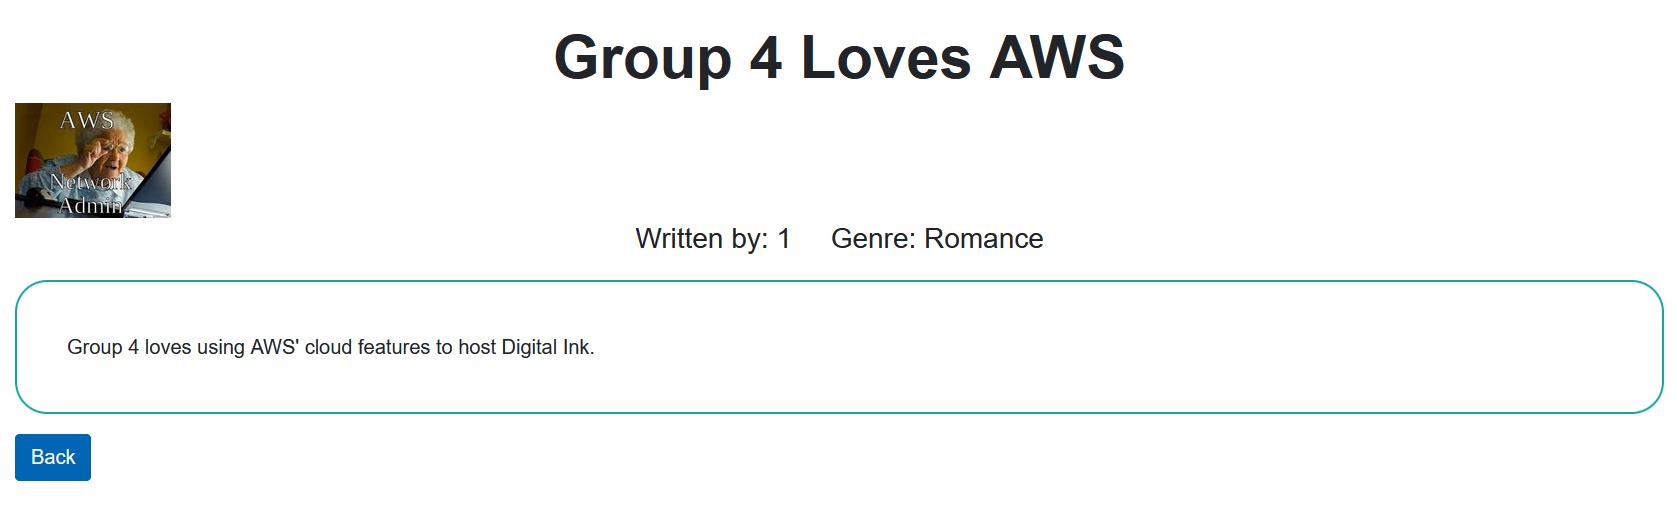
\includegraphics[width=\textwidth]{resources/webapp/digital-ink-story}
    \end{subfigure}
    \caption{\textit{Digital-Ink} stories page and story view.}
    \label{fig:digital-ink-stories-and-story}
\end{figure}
